% General params
\newcommand{\mainLineWidth}{1}
\newcommand{\embedLineWidth}{2}
\newcommand{\bigDeltaY}{1}
\newcommand{\smallDeltaY}{0.5}
\newcommand{\offsetY}{0.5}


% objrel
\newcommand{\objrelX}{0}
\newcommand{\objrelY}{0}
\newcommand{\objrelMainSubjectX}{-3}
\newcommand{\objrelMainVerbX}{2}
\newcommand{\objrelEmbedSubjectX}{-0.5}
\newcommand{\objrelEmbedVerbX}{0.9}

% mental-SR
\newcommand{\mentalSRX}{0}
\newcommand{\mentalSRY}{-3}
\newcommand{\mentalSRMainSubjectX}{-2.7}
\newcommand{\mentalSRMainVerbX}{-1.6}
\newcommand{\mentalSREmbedSubjectX}{0.5}
\newcommand{\mentalSREmbedVerbX}{1.8}

% objrel-nounpp
\newcommand{\objrelNounppX}{0}
\newcommand{\objrelNounppY}{-6}
\newcommand{\objrelNounppMainSubjectX}{-4}
\newcommand{\objrelNounppMainVerbX}{3.5}
\newcommand{\objrelNounppEmbedSubjectX}{-1.8}
\newcommand{\objrelNounppEmbedVerbX}{2.2}

% mental-LR
\newcommand{\mentalLRX}{0}
\newcommand{\mentalLRY}{-9}
\newcommand{\mentalLRMainSubjectX}{-4}
\newcommand{\mentalLRMainVerbX}{-2.8}
\newcommand{\mentalLREmbedSubjectX}{-0.8}
\newcommand{\mentalLREmbedVerbX}{3.2}


\begin{figure*}
\centering
\makebox[5cm][c]{%
\begin{minipage}{.9\textwidth}
    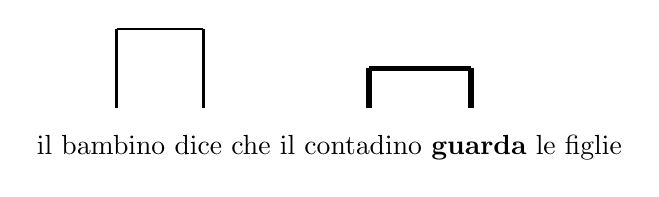
\begin{tikzpicture}
        % Sentence
        \node[align=left] at (\mentalSRX,\mentalSRY) {il bambino dice che il contadino \textbf{guarda} le figlie};
        
        % Draw main dependency
        \draw [line width=\mainLineWidth, black] (\mentalSRX+\mentalSRMainSubjectX,\mentalSRY+\offsetY) -- (\mentalSRX+\mentalSRMainSubjectX,\mentalSRY+\offsetY+\bigDeltaY);
        \draw [line width=\mainLineWidth, black] (\mentalSRX+\mentalSRMainSubjectX,\mentalSRY+\offsetY+\bigDeltaY) -- (\mentalSRX+\mentalSRMainVerbX,\mentalSRY+\offsetY+\bigDeltaY);
        \draw [line width=\mainLineWidth, black] (\mentalSRX+\mentalSRMainVerbX,\mentalSRY+\offsetY+\bigDeltaY) -- (\mentalSRX+\mentalSRMainVerbX,\mentalSRY+\offsetY);
    
        % Draw embedded dependency
        \draw [line width=\embedLineWidth, black] (\mentalSRX+\mentalSREmbedSubjectX,\mentalSRY+\offsetY) -- (\mentalSRX+\mentalSREmbedSubjectX,\mentalSRY+\offsetY+\smallDeltaY);
        \draw [line width=\embedLineWidth, black] (\mentalSRX+\mentalSREmbedSubjectX,\mentalSRY+\offsetY+\smallDeltaY) -- (\mentalSRX+\mentalSREmbedVerbX,\mentalSRY+\offsetY+\smallDeltaY);
        \draw [line width=\embedLineWidth, black] (\mentalSRX+\mentalSREmbedVerbX,\mentalSRY+\offsetY+\smallDeltaY) -- (\mentalSRX+\mentalSREmbedVerbX,\mentalSRY+\offsetY);
    \end{tikzpicture}
\end{minipage}
}


\makebox[5cm][c]{%
\begin{minipage}{.9\textwidth}
    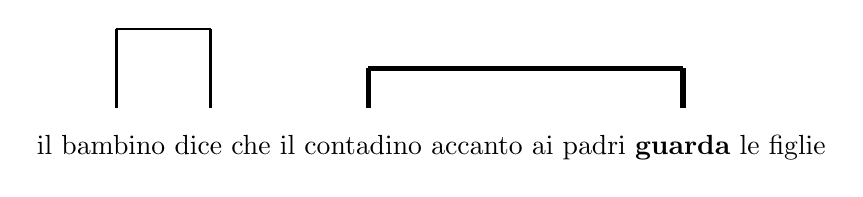
\begin{tikzpicture}
        % Sentence
        \node[align=left] at (\mentalLRX,\mentalLRY) {il bambino dice che il contadino accanto ai padri \textbf{guarda} le figlie};
        
        % Draw main dependency
        \draw [line width=\mainLineWidth, black] (\mentalLRX+\mentalLRMainSubjectX,\mentalLRY+\offsetY) -- (\mentalLRX+\mentalLRMainSubjectX,\mentalLRY+\offsetY+\bigDeltaY);
        \draw [line width=\mainLineWidth, black] (\mentalLRX+\mentalLRMainSubjectX,\mentalLRY+\offsetY+\bigDeltaY) -- (\mentalLRX+\mentalLRMainVerbX,\mentalLRY+\offsetY+\bigDeltaY);
        \draw [line width=\mainLineWidth, black] (\mentalLRX+\mentalLRMainVerbX,\mentalLRY+\offsetY+\bigDeltaY) -- (\mentalLRX+\mentalLRMainVerbX,\mentalLRY+\offsetY);
    
        % Draw embedded dependency
        \draw [line width=\embedLineWidth, black] (\mentalLRX+\mentalLREmbedSubjectX,\mentalLRY+\offsetY) -- (\mentalLRX+\mentalLREmbedSubjectX,\mentalLRY+\offsetY+\smallDeltaY);
        \draw [line width=\embedLineWidth, black] (\mentalLRX+\mentalLREmbedSubjectX,\mentalLRY+\offsetY+\smallDeltaY) -- (\mentalLRX+\mentalLREmbedVerbX,\mentalLRY+\offsetY+\smallDeltaY);
        \draw [line width=\embedLineWidth, black] (\mentalLRX+\mentalLREmbedVerbX,\mentalLRY+\offsetY+\smallDeltaY) -- (\mentalLRX+\mentalLREmbedVerbX,\mentalLRY+\offsetY);
    \end{tikzpicture}
\end{minipage}
}%


\makebox[5cm][c]{%
\begin{minipage}{.9\textwidth}
     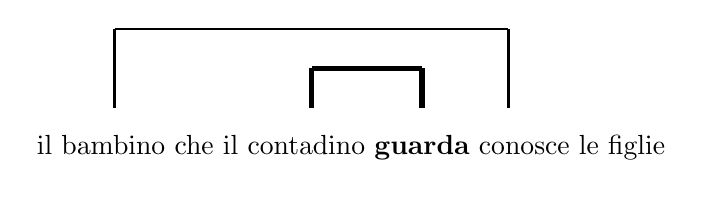
\begin{tikzpicture}
        % Sentence
        \node[align=left] at (\objrelX,\objrelY) {il bambino che il contadino \textbf{guarda} conosce le figlie};
        
        % Draw main dependency
        \draw [line width=\mainLineWidth, black] (\objrelX+\objrelMainSubjectX,\objrelY+\offsetY) -- (\objrelX+\objrelMainSubjectX,\objrelY+\offsetY+\bigDeltaY);
        \draw [line width=\mainLineWidth, black] (\objrelX+\objrelMainSubjectX,\objrelY+\offsetY+\bigDeltaY) -- (\objrelX+\objrelMainVerbX,\objrelY+\offsetY+\bigDeltaY);
        \draw [line width=\mainLineWidth, black] (\objrelX+\objrelMainVerbX,\objrelY+\offsetY+\bigDeltaY) -- (\objrelX+\objrelMainVerbX,\objrelY+\offsetY);
    
        % Draw embedded dependency
        \draw [line width=\embedLineWidth, black] (\objrelX+\objrelEmbedSubjectX,\objrelY+\offsetY) -- (\objrelX+\objrelEmbedSubjectX,\objrelY+\offsetY+\smallDeltaY);
        \draw [line width=\embedLineWidth, black] (\objrelX+\objrelEmbedSubjectX,\objrelY+\offsetY+\smallDeltaY) -- (\objrelX+\objrelEmbedVerbX,\objrelY+\offsetY+\smallDeltaY);
        \draw [line width=\embedLineWidth, black] (\objrelX+\objrelEmbedVerbX,\objrelY+\offsetY+\smallDeltaY) -- (\objrelX+\objrelEmbedVerbX,\objrelY+\offsetY);
    \end{tikzpicture}
\end{minipage}
}%


\makebox[5cm][c]{%
\begin{minipage}{.9\textwidth}
    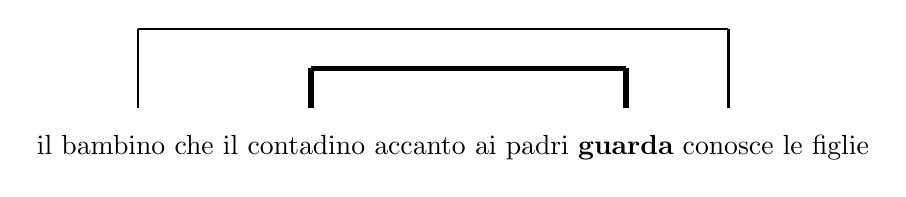
\begin{tikzpicture}
        % Sentence
        \node[align=left] at (\objrelNounppX,\objrelNounppY) {il bambino che il contadino accanto ai padri \textbf{guarda} conosce le figlie};
        
        % Draw main dependency
        \draw [line width=\mainLineWidth, black] (\objrelNounppX+\objrelNounppMainSubjectX,\objrelNounppY+\offsetY) -- (\objrelNounppX+\objrelNounppMainSubjectX,\objrelNounppY+\offsetY+\bigDeltaY);
        \draw [line width=\mainLineWidth, black] (\objrelNounppX+\objrelNounppMainSubjectX,\objrelNounppY+\offsetY+\bigDeltaY) -- (\objrelNounppX+\objrelNounppMainVerbX,\objrelNounppY+\offsetY+\bigDeltaY);
        \draw [line width=\mainLineWidth, black] (\objrelNounppX+\objrelNounppMainVerbX,\objrelNounppY+\offsetY+\bigDeltaY) -- (\objrelNounppX+\objrelNounppMainVerbX,\objrelNounppY+\offsetY);
    
        % Draw embedded dependency
        \draw [line width=\embedLineWidth, black] (\objrelNounppX+\objrelNounppEmbedSubjectX,\objrelNounppY+\offsetY) -- (\objrelNounppX+\objrelNounppEmbedSubjectX,\objrelNounppY+\offsetY+\smallDeltaY);
        \draw [line width=\embedLineWidth, black] (\objrelNounppX+\objrelNounppEmbedSubjectX,\objrelNounppY+\offsetY+\smallDeltaY) -- (\objrelNounppX+\objrelNounppEmbedVerbX,\objrelNounppY+\offsetY+\smallDeltaY);
        \draw [line width=\embedLineWidth, black] (\objrelNounppX+\objrelNounppEmbedVerbX,\objrelNounppY+\offsetY+\smallDeltaY) -- (\objrelNounppX+\objrelNounppEmbedVerbX,\objrelNounppY+\offsetY);
    \end{tikzpicture}
\end{minipage}
}%
    %         \end{tikzpicture}
    \caption{Design} 
\end{figure*}
    